

\lecture{11}{2024-10-15}{Inverse de Matrice et déterminant}



\paragraph{La matrice des cofacteurs} Soit $A$ une matrice $n \times n$ et $A_{ij}$ la matrice $(n-1) \times (n-1)$ obtenue en supprimant la $i^{eme}$ ligne et la $j^{eme}$ colonne de $A$.
\\
\begin{exemple}
    Si on prend la matrice $A = \begin{pmatrix}
        1 & 2 & 3 \\
        4 & 5 & 6 \\
        7 & 8 & 9
    \end{pmatrix}$ et qu'on prend $A_{23}$, alors on enlève la ligne 2 et la colonne 3 ce qui donne que 
    \[ A_{23} = \begin{pmatrix}
        1 & 2 \\
        7 & 8
    \end{pmatrix}\]
    \begin{definition}
        Le \textbf{cofacteur} $C_{ij} = (-1)^{i+j}det A_{ij}$.
    \end{definition}
\end{exemple}
\begin{definition}
    
    La \textbf{comatrice} ou \textbf{matrice des cofacteurs} de $A$ est la matrice
    \[ComA = (C_{ij})_{n\times n}\]
\end{definition}

\paragraph{Cofacteur et inverse}
Soit $A$ une matrice $n \times n$ inversible. On pose:
\[A_j(\vec{e}_i) = (\vec{a}_1 ... \vec{a}_{j-1} \vec{e}_i \vec{a}_{j+1} ... \vec{a}_n)\]
La seule solution du système $A\vec{x} = \vec{e}_i$ est donnée par la formule:
\begin{definition}[Formules de Cramer]
    \begin{equation*}
        x_j = \frac{\det A_j(\vec{e}_i)}{\det A}
    \end{equation*}
\end{definition}


De plus, en développant le déterminant selon la $j^{eme}$ colonne on calcule:
\[\det A_j(\vec{e}_i) = (-1)^{i+j}\det A_{ij}\]

\paragraph{Formule pour l'inverse}
\begin{definition}
    \begin{equation*}
        A^{-1} = \frac{1}{\det A}(ComA)^t
    \end{equation*}
\end{definition}
En français, la matrice inverse est donnée par la transposée des cofacteurs multiplié par l'inverse du déterminant.

\begin{exemple}
    Prenons une matrice $2 \times 2$:
    \[ \begin{vmatrix}
        a & b \\
        c & d
    \end{vmatrix}
    \]
    On a donc:
    \begin{itemize}
        \item $C_{11} = (-1)^{1+1}\det(d) = d$
        \item $C_{21} = (-1)^{2+1}\det(b) = -b$
        \item $C_{12} = (-1)^{1+2}\det(c) = -c$
        \item $C_{22} = (-1)^{2+2}\det(d) = a$
    \end{itemize}
\end{exemple}
Par conséquent $A^{-1}$ est la seule solution du sytème $A\vec{x} = \vec{e}_i$ qui est donné par la formule:
\begin{formule}

\[
    x_j = \frac{\det A_j (\vec{e}_i)}{\det A} = \frac{(-1)^{i+j}\det A_{ij}}{\det A} = \frac{C_{ij}}{\det A}
\]
\end{formule}
\\
On calcule la $i^{eme}$ colonne de la matrice $A\cdot\frac{1}{\det A}(ComA)^T$:
\[
A\cdot \frac{1}{\det A}\begin{pmatrix}
    C_{i1}\\
    .\\
    . \\
    . \\
    C_{in}
    
\end{pmatrix} = A\vec{x} = \vec{e}_i
\]

\begin{exemple}

    Soit $A = \begin{pmatrix}
        1 & 1 & 1 & 0\\
        0 & 3 & 1 & 2\\
        2 & 3 & 1 & 0 \\
        1 & 0 & 2 & 1
    \end{pmatrix}$
\\
Alors: $\det A = \begin{vmatrix}
        1 & 1 & 1 & 0\\
        0 & 3 & 1 & 2\\
        2 & 3 & 1 & 0 \\
        1 & 0 & 2 & 1
\end{vmatrix}$ = $\begin{vmatrix}
        1 & 0 & 0 & 0\\
        0 & 3 & 1 & 2\\
        2 & 1 & -1 & 0 \\
        1 & -1 & 1 & 1
        \end{vmatrix}$ \hspace{0.4cm} on peut prendre le cofacteur de $A_{11}$: 
        $1\cdot \begin{vmatrix}
        3 & 1 & 2\\
        1 & -1 & 0 \\
        -1 & 1 & 1
        \end{vmatrix}$
        $=(-1)^{1+1} \begin{vmatrix}
            3 & 1 & 2 \\
            1 & -1 & 0 \\
            0 & 0 & 1
        \end{vmatrix}$ si on dévelope selon le 1 en bas à gauche:
        $  (-1)^{3+3} \begin{vmatrix}
            3 & 1 \\
            1 & -1
        \end{vmatrix} = -4$

        \\
        \\
        Prenons maintenant:
        \[|A_{32}| = \begin{vmatrix}
            1 & 1 & 0 \\
            0 & 1 & 2\\
            1 & 2 & 1
        \end{vmatrix} = \dots = -1\]
        \subparagraph{Conclusion:} 
        \[b_{23} = \frac{1}{\det A}\cdot(ComA)^T = \frac{C_{32}}{\det A}\]
        \[= \frac{(-1)^{2+3}\cdot \det A_{23}}{\det A}\]
        \[b_{23} = -\frac{1}{4}\]
\end{exemple}
\paragraph{Aire d'un parallélogramme}
Soit $\begin{pmatrix} a \\ c \end{pmatrix}$ et $\begin{pmatrix} b \\ d \end{pmatrix}$ deux vecteur de \R$^2$ et $A = \begin{pmatrix}
    a & b \\
    c & d
\end{pmatrix}$
\begin{theorem}
    L'aire du parallélogramme construit sur $\begin{pmatrix} a \\ c \end{pmatrix}$ et $\begin{pmatrix} b \\ d \end{pmatrix}$ vaut $|\det A|$.
\end{theorem}

\subparagraph{Preuve.}
Quitte  échanger les vecteur $\vec{u}$ et $\vec{v}$ (resp. les colonnes de $A$), on peut supposer que $a_{11} \neq 0$ sans changer l'aire du parallélogramme (resp. sans changer la valeur absolue de $\det A$).
\\
En effectuant une opération de type I sur les colonnes de $A$ on obtient $0$ sur $a_{12}$ sans changer $\det A$, ni l'aire du parallélogramme.
\\
En effectuant une deuxième opération de type I sur les colonne de A, on se retrouve à une matrice $\begin{pmatrix}
    \alpha & 0\\
    0 & \beta
\end{pmatrix}$ le $\det$ vaut $\alpha \cdot \beta$, c'est l'aire du rectangle construit sur $\alpha \cdot \hat{e}_1$, $\beta\cdot\hat{e}_2$

\begin{exemple}
Prenons les points $A(1, 2), B(4, 3), C(8, 1), D(5, -1)$
\\
\begin{center}
    
        
    
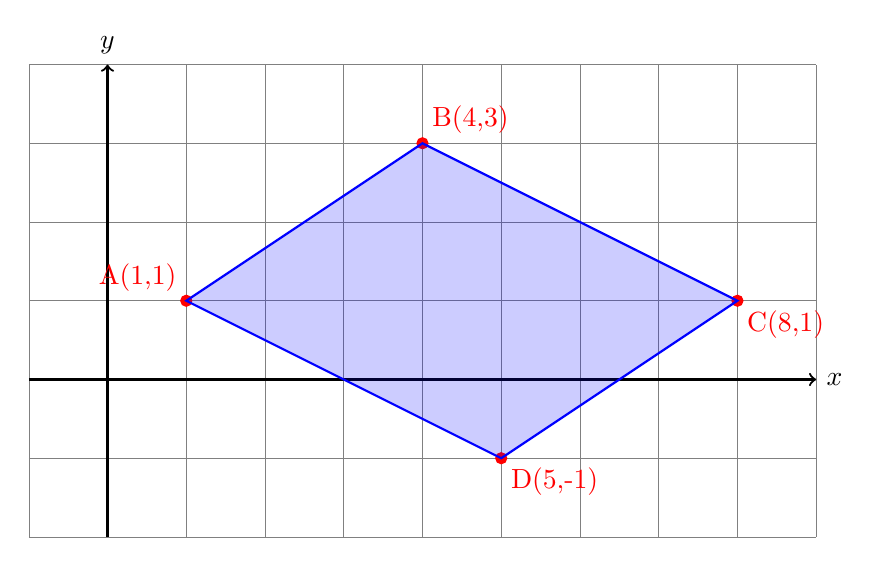
\begin{tikzpicture}
    % Grille de fond
    \draw[step=1cm, gray, very thin] (-1,-2) grid (9,4);

    % Axes
    \draw[thick,->] (-1,0) -- (9,0) node[right] {$x$};
    \draw[thick,->] (0,-2) -- (0,4) node[above] {$y$};

    % Points A, B, C, D
    \filldraw[red] (1,1) circle (2pt) node[above left] {A(1,1)};
    \filldraw[red] (4,3) circle (2pt) node[above right] {B(4,3)};
    \filldraw[red] (8,1) circle (2pt) node[below right] {C(8,1)};
    \filldraw[red] (5,-1) circle (2pt) node[below right] {D(5,-1)};
   % Surlignage du parallélogramme
    \fill[blue, opacity=0.2] (1,1) -- (4,3) -- (8,1) -- (5,-1) -- cycle;

    % Lignes reliant les points
    \draw[thick, blue] (1,1) -- (4,3) -- (8,1) -- (5,-1) -- cycle;

\end{tikzpicture}


\end{center}

On a donc que Aire$(\beta) = \left|\det (\vec{AB}, \vec{AD})\right| = \left|\det \begin{pmatrix}
    3 & 4 \\ 2 & -2
\end{pmatrix}\right| = 14$
\end{exemple}


\subparagraph{Aire et application linéaire}
Une application linéaire $T : \mathbb{R}^2 \to \mathbb{R}^2$ transforme les vecteurs $\vec{e}_1$ et $\vec{e}_2$ en deux vecteur u et v. Ainsi $T$ transforme les carré unité de sommets



\begin{theorem}
    Soit $T : \mathbb{R}^2 \to \mathbb{R}^2$  une application linéaire représentée par la matrice $A$. Soit $S$ une région du plan alors:
\begin{formule}
    \[Aire(T(S)) = |\det A| \cdot Aire(S)\]
\end{formule}
\end{theorem}
\begin{framedremark}
    L'aire d'un prallélogramme ou le volume d'un parraéélépiède ne dépendent que des vecteurs qui les supportent. L'un des sommets peut être l'origine ou non. L'aire et le volume sont \textbf{invariants par translation}.
\end{framedremark}
\begin{exemple}
    On cherche l'aire de l'ellipse d'équation$\frac{x^2}{a^2} + \frac{y^2}{b^2} = 1$
    \\
    L'application est:
    \[T: \mathbb{R}^2 \to \mathbb{R}^2 \]
    \[\begin{pmatrix}
        x \\ y
    \end{pmatrix} \to \begin{pmatrix}
        ax \\ by
    \end{pmatrix}\]
    La matrice est donc: 
    \[\begin{pmatrix}
        a & 0\\ 0 & b
    \end{pmatrix}\]
    \\
    Le cercle unité $e$ d'équation $x^2 + y^2 ) 1$ est transformé en $\epsilon$ par $T$. Si $(x, y) \in e$:
    \[T\begin{pmatrix}
        x \\ y
    \end{pmatrix} = \begin{pmatrix}
        ax \\ by
    \end{pmatrix} \in \epsilon\] car $\frac{(ax)^2}{a^2} + \frac{(by)^2}{b^2} = x^2 + y^2$
    \\
    Aire($\epsilon$) $= \det \begin{pmatrix}
        a & 0 \\ 0 & b
    \end{pmatrix} \cdot Aire(e) = \pi\cdot a \cdot b$
\end{exemple}




